% ============================================================
% Figure: Conceptual station heatmap
% ============================================================
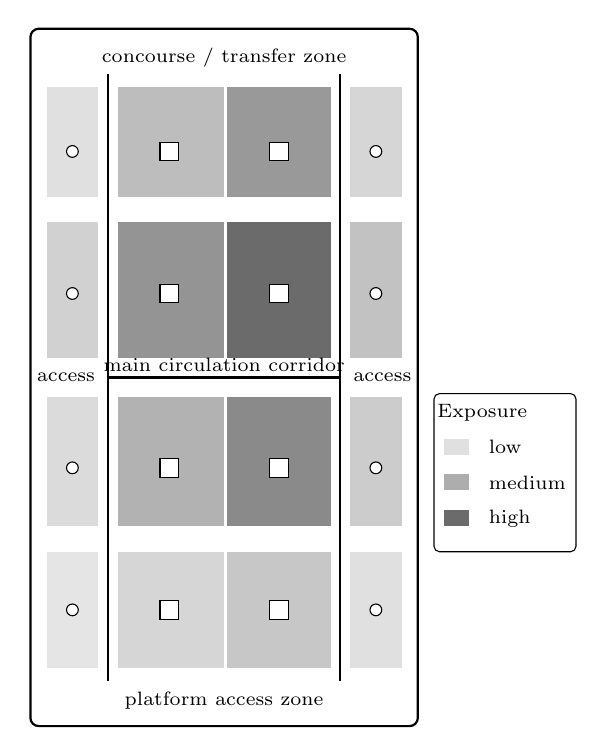
\begin{tikzpicture}[
    x=0.82cm,
    y=0.82cm,
    font=\small
]

% Outer boundary
\draw[rounded corners=3pt, thick] (0,0) rectangle (6,10.8);

% Main spatial structure
\draw[thick] (1.2,0.7) -- (1.2,10.1);
\draw[thick] (4.8,0.7) -- (4.8,10.1);
\draw[thick] (1.2,5.4) -- (4.8,5.4);

% Heatmap cells
\fill[black!10] (0.25,0.9) rectangle (1.05,2.7);
\fill[black!16] (1.35,0.9) rectangle (3.0,2.7);
\fill[black!22] (3.05,0.9) rectangle (4.65,2.7);
\fill[black!12] (4.95,0.9) rectangle (5.75,2.7);

\fill[black!14] (0.25,3.1) rectangle (1.05,5.1);
\fill[black!30] (1.35,3.1) rectangle (3.0,5.1);
\fill[black!46] (3.05,3.1) rectangle (4.65,5.1);
\fill[black!20] (4.95,3.1) rectangle (5.75,5.1);

\fill[black!18] (0.25,5.7) rectangle (1.05,7.8);
\fill[black!42] (1.35,5.7) rectangle (3.0,7.8);
\fill[black!58] (3.05,5.7) rectangle (4.65,7.8);
\fill[black!24] (4.95,5.7) rectangle (5.75,7.8);

\fill[black!12] (0.25,8.2) rectangle (1.05,9.9);
\fill[black!26] (1.35,8.2) rectangle (3.0,9.9);
\fill[black!40] (3.05,8.2) rectangle (4.65,9.9);
\fill[black!16] (4.95,8.2) rectangle (5.75,9.9);

% Devices
\foreach \x/\y in {0.65/1.8,0.65/4.0,0.65/6.7,0.65/8.9,5.35/1.8,5.35/4.0,5.35/6.7,5.35/8.9}
    \node[circle, draw, fill=white, inner sep=1.5pt] at (\x,\y) {};

\foreach \x/\y in {2.15/1.8,3.85/1.8,2.15/4.0,3.85/4.0,2.15/6.7,3.85/6.7,2.15/8.9,3.85/8.9}
    \node[rectangle, draw, fill=white, minimum width=0.14cm, minimum height=0.14cm] at (\x,\y) {};

% Labels
\node[font=\scriptsize] at (3,10.35) {concourse / transfer zone};
\node[font=\scriptsize] at (3,5.6) {main circulation corridor};
\node[font=\scriptsize] at (3,0.4) {platform access zone};
\node[font=\scriptsize] at (0.55,5.4) {access};
\node[font=\scriptsize] at (5.45,5.4) {access};

% Minimal legend
\draw[rounded corners=2pt] (6.25,2.7) rectangle (8.45,5.15);
\node[font=\scriptsize] at (7,4.85) {Exposure};

\fill[black!12] (6.4,4.2) rectangle (6.8,4.45);
\node[anchor=west, font=\scriptsize] at (6.95,4.32) {low};

\fill[black!32] (6.4,3.65) rectangle (6.8,3.9);
\node[anchor=west, font=\scriptsize] at (6.95,3.77) {medium};

\fill[black!58] (6.4,3.1) rectangle (6.8,3.35);
\node[anchor=west, font=\scriptsize] at (6.95,3.22) {high};

\end{tikzpicture}